\documentclass[12pt,twoside]{article}

\usepackage{amsmath}

\usepackage{times}
\usepackage{helvet}

%\usepackage{fontspec}
%\setmainfont{Liberation Serif}
%\setsansfont{Liberation Sans}

\usepackage{geometry}
\geometry{               
	letterpaper,
	bottom=0.5in,
	top=0.5in,
	inner=1in,
	outer=0.5in,
        footskip=4ex
}

\usepackage{graphicx}

\usepackage{titling}
\pretitle{\begin{center}\LARGE\sffamily}
\posttitle{\par\end{center}\vspace{-4ex}}
\preauthor{\begin{center}\large\sffamily}
\postauthor{\par\end{center}\vspace{-12ex}}
\setlength{\droptitle}{-60pt}



\usepackage{multienum}

\usepackage{titlesec}
\titleformat*{\section}{\Large\sffamily}
\titleformat*{\subsection}{\sffamily}

\titlespacing\section{2em}{0.5ex plus 0.2ex minus 0.1ex}{0pt}
\titlespacing\subsection{1em}{0.5ex plus 0.2ex minus 0.1ex}{0pt}

\usepackage{fancyhdr}
\pagestyle{fancy}

\fancyhf{}
\renewcommand{\headrule}{}
\fancyfoot[LE]{\thepage}
\fancyfoot[RO]{\thepage}

\usepackage{multicol}

\setlength{\parindent}{0pt}


\title{Lesson 30}
\author{Foundations of College Algebra}
\date{}

\begin{document}

\maketitle

\thispagestyle{fancy}
\section*{Review}

\begin{enumerate}
	\item Simplify. $$\sqrt{36}\div\sqrt{9}+2^2\cdot7-17$$ \vspace\fill
	\item Find the prime factorization of the following number. Write any repeated factors using exponents. $$588$$ \vspace\fill
	\item Multiply. Write the answer in simplest form. $$1 \frac16\cdot \frac6{49}$$ \vspace\fill
	\item Divide. Write your answer in simplest form. $$ \frac2{33} \div \frac{10}{143}$$ \vspace\fill
	\item Add and simplify. $$\frac3{66} + \frac3{55}$$ \vspace\fill \pagebreak
	\item A landscape architect is planning a border for a flower garden shaped like a triangle.
		The sides of the garden measure 16.2 feet, 24.66 feed, and 22.8 feet. Find the amount of border material needed.\\
	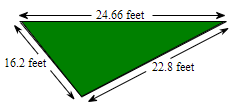
\includegraphics[height=1.5in]{FinalTriangle.png}
	\item A self-tanning lotion advertises that a 2-oz bottle will provide four applications. Jen found a great deal on a 13-oz bottle of the self-tanning lotion she had been using. Based on advertising claims, how many applications of the self-tanner should Jen expect?\vspace\fill
	\item In 1999, total revenue of a music company from music sales and licensing was \$14.3 billion. It was forecasted that this number would continue to drop until it reached \$5.5 billion in 2014. Find this percent decrease in music revenue.\vspace\fill
	\item The sales tax is \$115.50 on a stereo system purchase of \$1650. Find the sales tax rate. \vspace\fill
	\item Sketch the right triangle and find the length of the side not given. (Each length is in units.) $$\text{leg}=10 \text{, leg}=12$$ \vspace\fill \pagebreak
	\item Decide whether the given number is a solution of the given equation. $$ \frac{x}2 - 1= -2; \qquad x=6$$ \vspace\fill
	\item Solve the equation. $$-4(n-2)=6-3n$$ \vspace\fill
	\item Solve the equation. $$6x+1=9x+7$$ \vspace\fill
	\item Solve the equation for $x$. $$ \frac34 x - \frac12=7$$ \vspace\fill \pagebreak
	\item Solve the inequality. Write your answer in set notation. $$8(x+1)-7x\geq-5$$ \vspace\fill
	\item Graph the linear equation. $x+1=0$ \\
 	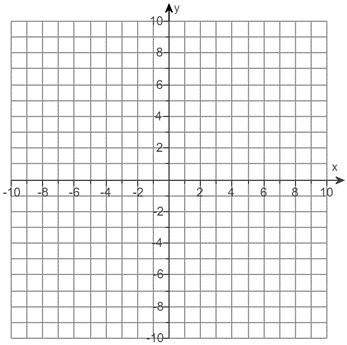
\includegraphics[height=3in]{GraphPaper.png}
	\item Write an equation of the line with the given slope, $m$, and $y$-intercept $(0,b)$. $$ m=-\frac34 \text{, } b=\frac12$$ \vspace\fill
	\item Use the product rule to simplify the expression. Write the results using exponents. $$(4z^{11} )(-6z^8 )(z^2 )$$ \vspace\fill \pagebreak
	\item Subtract. $$(4z^2-10z+7)-(10z^2+2z-9)$$ \vspace\fill
	\item Multiply using the FOIL method. $$(y^2+4)(2y+5)$$ \vspace\fill
	\item Factor the trinomial completely. $$x^2-x-42$$ \vspace\fill
	\item Solve the equation. $$x^2-13x+36=0$$ \vspace\fill
\end{enumerate}

\end{document}
